% Time structure of el1xr_opt: one timeline in 1-minute base units, a resolution for each asset
% and flow, and the constraint resolutions derived from them (Gao et al., Applied Energy 396
% (2025) 126267, Algorithms 1 and 2).
%
% Build:  pdflatex el1xr_opt_time_structure.tex
%         pdftocairo -svg el1xr_opt_time_structure.pdf ../el1xr_opt_time_structure.svg
\documentclass[tikz,border=6pt]{standalone}
\usepackage[scaled]{helvet}
\renewcommand{\familydefault}{\sfdefault}
\usepackage{sansmath}
\sansmath
\hyphenpenalty=10000 \exhyphenpenalty=10000 \pretolerance=-1
\usetikzlibrary{positioning,decorations.pathreplacing,calc}

% palette of docs/img/el1xr_opt_architecture.svg
\definecolor{ink}{HTML}{111827}
\definecolor{muted}{HTML}{555555}
\definecolor{bluefill}{HTML}{E8F1FC}  \definecolor{bluedraw}{HTML}{3B6FB6}
\definecolor{greenfill}{HTML}{E7F6EA} \definecolor{greendraw}{HTML}{3C8D4F}
\definecolor{orangefill}{HTML}{FDF3E3}\definecolor{orangedraw}{HTML}{C07A1E}
\definecolor{violetfill}{HTML}{F0EAFB}\definecolor{violetdraw}{HTML}{6E4BB5}
\definecolor{greyfill}{HTML}{F3F4F6}

\begin{document}
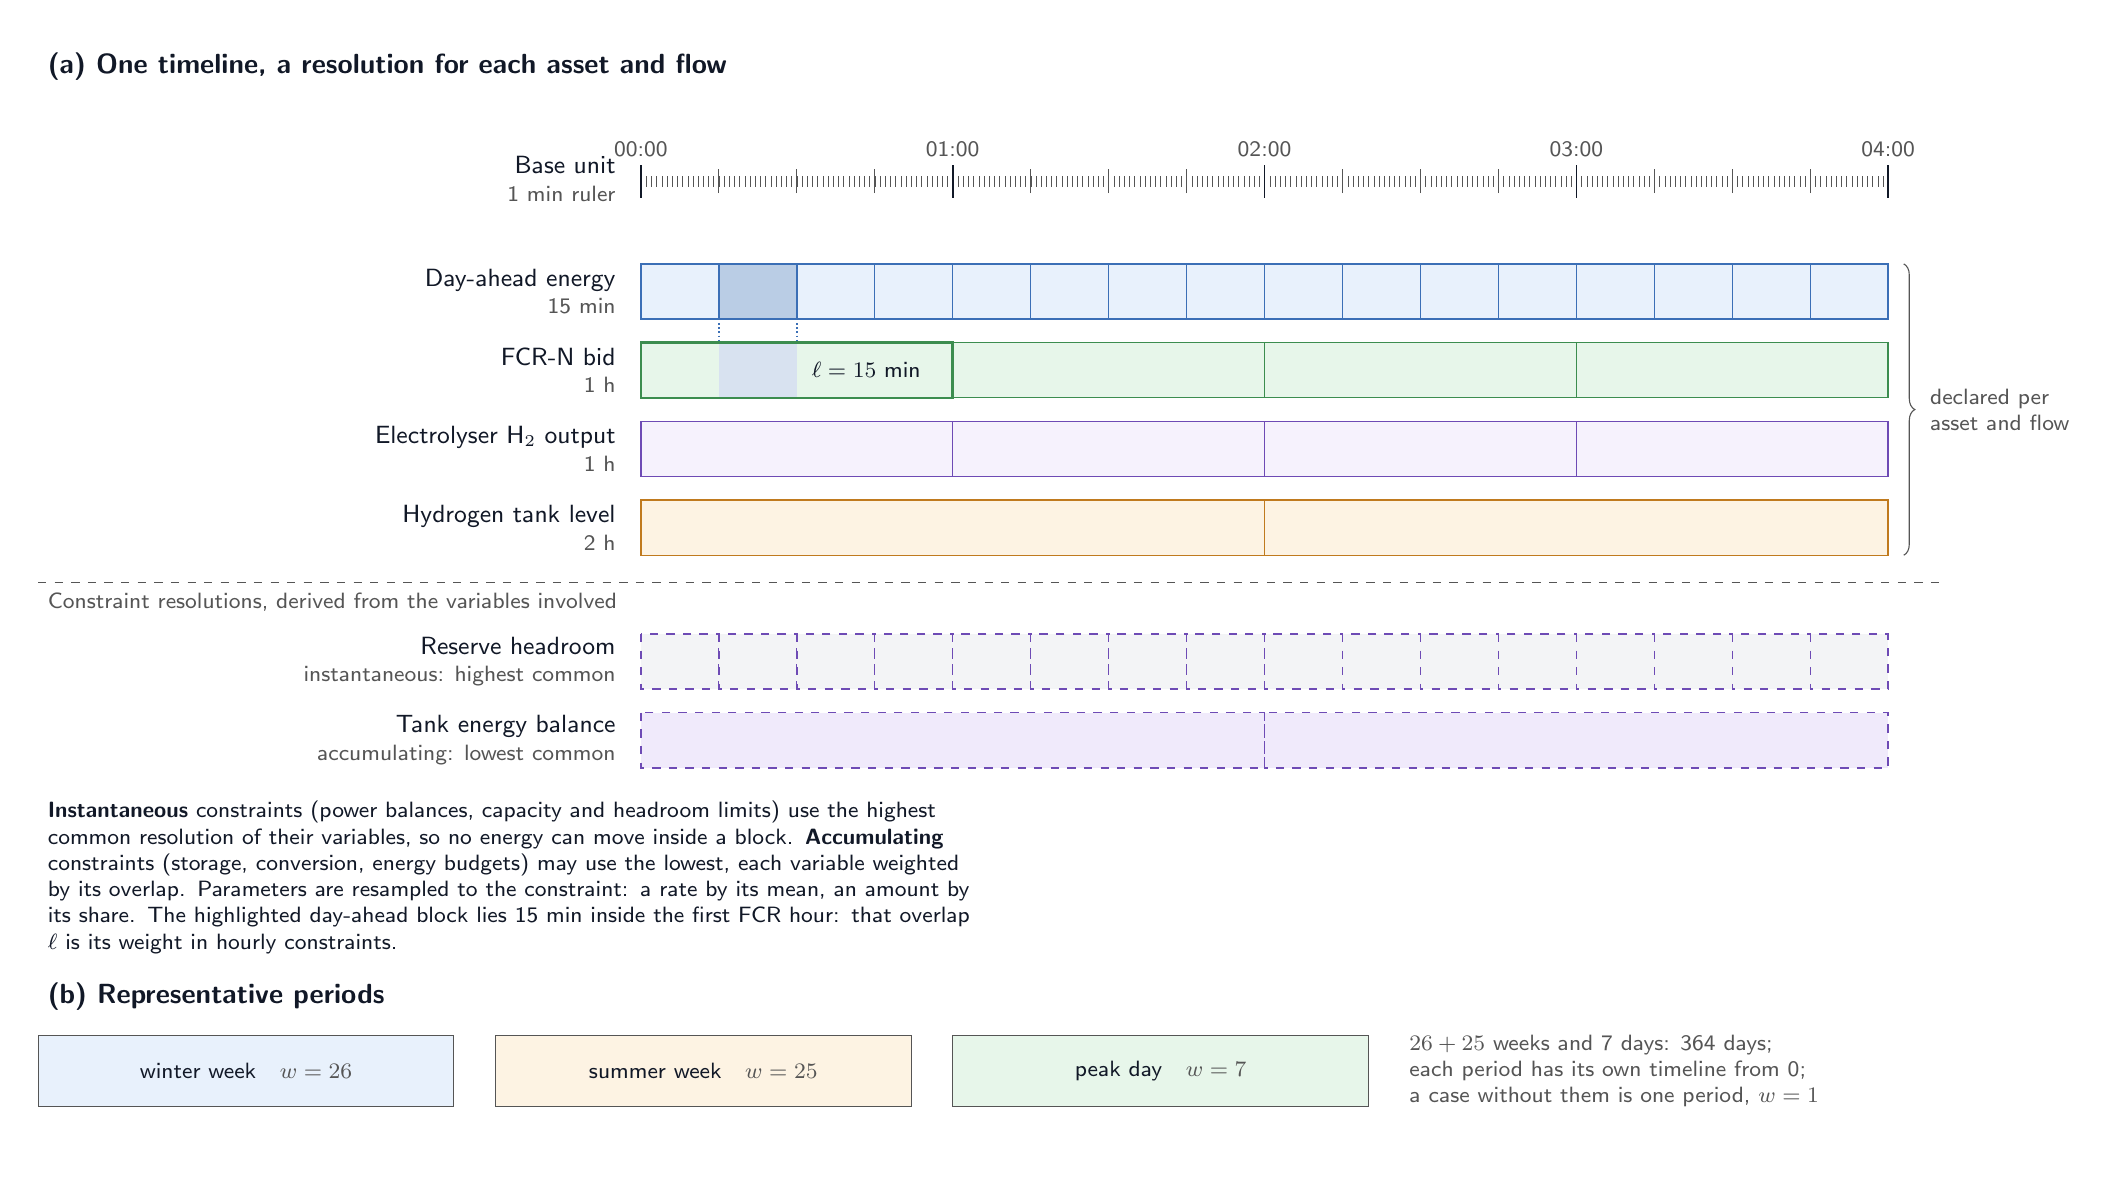
\begin{tikzpicture}[x=0.66mm, y=1mm, font=\small, text=ink,
    blk/.style={draw=#1, line width=0.5pt},
    lab/.style={anchor=east, align=right, font=\small},
    sub/.style={font=\footnotesize, text=muted}]

  % background, so the figure reads on dark pages too
  \fill[white] (-118,-124) rectangle (252,20);

  % ---------------- panel (a): resolutions on one timeline ----------------
  \node[anchor=west, font=\bfseries] at (-116,15) {(a) One timeline, a resolution for each asset and flow};

  % time axis, 0..240 base units (1 min each)
  \def\rowh{7}
  % row y positions (top of each row)
  \def\yruler{2}  \def\yda{-10} \def\yfcr{-20} \def\yely{-30} \def\ytank{-40}
  \def\yinst{-57} \def\yacc{-67}

  % 1-min ruler: a tick every minute, longer every 15 min and every hour
  \node[lab] at (-3,\yruler-1.2) {Base unit\\[-1pt]\footnotesize\color{muted}1 min ruler};
  \foreach \t in {0,1,...,240} {\draw[muted, line width=0.12pt] (\t,\yruler-2.2) -- (\t,\yruler-0.8);}
  \foreach \t in {0,15,...,240} {\draw[muted, line width=0.4pt] (\t,\yruler-3) -- (\t,\yruler);}
  \foreach \t/\l in {0/00:00,60/01:00,120/02:00,180/03:00,240/04:00} {
    \draw[ink, line width=0.6pt] (\t,\yruler-3.6) -- (\t,\yruler+0.6);
    \node[sub, above] at (\t,\yruler+0.4) {\l};}

  % day-ahead energy, 15 min
  \node[lab] at (-3,\yda-\rowh/2) {Day-ahead energy\\[-1pt]\footnotesize\color{muted}15 min};
  \foreach \s in {0,15,...,225} {\filldraw[fill=bluefill, blk=bluedraw] (\s,\yda) rectangle ++(15,-\rowh);}

  % FCR-N bid, 1 h
  \node[lab] at (-3,\yfcr-\rowh/2) {FCR-N bid\\[-1pt]\footnotesize\color{muted}1 h};
  \foreach \s in {0,60,...,180} {\filldraw[fill=greenfill, blk=greendraw] (\s,\yfcr) rectangle ++(60,-\rowh);}

  % electrolyser hydrogen output, 1 h
  \node[lab] at (-3,\yely-\rowh/2) {Electrolyser H$_2$ output\\[-1pt]\footnotesize\color{muted}1 h};
  \foreach \s in {0,60,...,180} {\filldraw[fill=violetfill!60, blk=violetdraw] (\s,\yely) rectangle ++(60,-\rowh);}

  % hydrogen tank level, 2 h
  \node[lab] at (-3,\ytank-\rowh/2) {Hydrogen tank level\\[-1pt]\footnotesize\color{muted}2 h};
  \foreach \s in {0,120} {\filldraw[fill=orangefill, blk=orangedraw] (\s,\ytank) rectangle ++(120,-\rowh);}

  % brace: declared per asset and flow
  \draw[decorate, decoration={brace, amplitude=4pt}, muted] (243,\yda) -- (243,\ytank-\rowh)
    node[midway, right=6pt, align=left, font=\footnotesize, text=muted] {declared per\\asset and flow};

  % separator
  \draw[muted, dashed, line width=0.4pt] (-116,-50.5) -- (250,-50.5);
  \node[anchor=west, sub] at (-116,-53) {Constraint resolutions, derived from the variables involved};

  % instantaneous: highest common resolution of day-ahead and FCR (Algorithm 1)
  \node[lab] at (-3,\yinst-\rowh/2) {Reserve headroom\\[-1pt]\footnotesize\color{muted}instantaneous: highest common};
  \foreach \s in {0,15,...,225} {\filldraw[fill=greyfill, draw=violetdraw, dashed, line width=0.5pt] (\s,\yinst) rectangle ++(15,-\rowh);}

  % accumulating: lowest common resolution of electrolyser output and tank (Algorithm 2)
  \node[lab] at (-3,\yacc-\rowh/2) {Tank energy balance\\[-1pt]\footnotesize\color{muted}accumulating: lowest common};
  \foreach \s in {0,120} {\filldraw[fill=violetfill, draw=violetdraw, dashed, line width=0.5pt] (\s,\yacc) rectangle ++(120,-\rowh);}

  % overlap: day-ahead block 00:15-00:30 inside FCR hour 00:00-01:00
  \filldraw[fill=bluedraw!35, draw=bluedraw, line width=0.9pt] (15,\yda) rectangle ++(15,-\rowh);
  \fill[bluedraw!20] (15,\yfcr) rectangle ++(15,-\rowh);
  \draw[greendraw, line width=0.9pt] (0,\yfcr) rectangle ++(60,-\rowh);
  \draw[bluedraw, line width=0.5pt, densely dotted] (15,\yda-\rowh) -- (15,\yfcr) (30,\yda-\rowh) -- (30,\yfcr);
  \node[font=\footnotesize, anchor=west] at (31,\yfcr-\rowh/2) {$\ell = 15$ min};

  % rule legend
  \node[anchor=north west, font=\footnotesize, align=left, text width=118mm] at (-116,-77)
    {\textbf{Instantaneous} constraints (power balances, capacity and headroom limits) use the highest
     common resolution of their variables, so no energy can move inside a block.
     \textbf{Accumulating} constraints (storage, conversion, energy budgets) may use the lowest,
     each variable weighted by its overlap. Parameters are resampled to the constraint: a rate by its
     mean, an amount by its share. The highlighted day-ahead block lies 15 min inside the first
     FCR hour: that overlap $\ell$ is its weight in hourly constraints.};

  % ---------------- panel (b): representative periods ----------------
  \node[anchor=west, font=\bfseries] at (-116,-103) {(b) Representative periods};
  \foreach \x/\n/\w/\c in {-116/winter week/$w = 26$/bluefill, -28/summer week/$w = 25$/orangefill, 60/peak day/$w = 7$/greenfill} {
    \filldraw[fill=\c, draw=muted, line width=0.4pt] (\x,-108) rectangle ++(80,-9);
    \node[font=\footnotesize, align=center] at (\x+40,-112.5) {\n\quad\color{muted}\w};}
  \node[anchor=west, font=\footnotesize, text=muted, align=left] at (146,-112.5)
    {$26 + 25$ weeks and 7 days: 364 days;\\each period has its own timeline from 0;\\a case without them is one period, $w = 1$};
\end{tikzpicture}
\end{document}
